\chapter{Sprint Planning}

\section*{User Stories and Implementations}

\begin{itemize}
	\item \textbf{Search for Points of Interest}
	\begin{itemize}
		\item As a user, I want to search for points of interest in a specific area.
		\item \textbf{Implementation:} Implement a search feature using a search bar where users can input keywords. Use a search algorithm to filter points of interest based on location and keyword matching.
		\item \textbf{Responsible:} Developer A
	\end{itemize}
	
	\item \textbf{Apply Filters}
	\begin{itemize}
		\item As a user, I want to filter search results by type, price, and rating.
		\item \textbf{Implementation:} Create UI elements for filtering options (type, price, rating). Implement logic to filter search results based on selected filters.
		\item \textbf{Responsible:} Developer B
	\end{itemize}
	
	\item \textbf{View Point of Interest Details}
	\begin{itemize}
		\item As a user, I want to view detailed information about a point of interest.
		\item \textbf{Implementation:} Design a details screen that displays a larger image of the point of interest, descriptive text, ratings, and user reviews. Retrieve and display specific data related to the selected point of interest.
		\item \textbf{Responsible:} Developer C
	\end{itemize}
	
	\item \textbf{Navigate Between Screens}
	\begin{itemize}
		\item As a user, I want to easily navigate between the home, account, and FAQ screens.
		\item \textbf{Implementation:} Set up a bottom navigation bar to switch between the home, account, and FAQ screens. Utilize navigation components or intents to navigate seamlessly.
		\item \textbf{Responsible:} Developer A
	\end{itemize}
	
	\item \textbf{View FAQ}
	\begin{itemize}
		\item As a user, I want to access a list of frequently asked questions and their answers.
		\item \textbf{Implementation:} Create a screen displaying a list of frequently asked questions and corresponding answers. Populate this screen with FAQ data retrieved from a data source.
		\item \textbf{Responsible:} Developer D
	\end{itemize}
	
	\item \textbf{View User Account Information}
	\begin{itemize}
		\item As a user, I want to view my profile information including a picture, name, email, and bio.
		\item \textbf{Implementation:} Develop an account screen with UI components displaying user profile information retrieved from the user's account settings.
		\item \textbf{Responsible:} Developer B
	\end{itemize}
	
	\item \textbf{Sign-up for an Account}
	\begin{itemize}
		\item As a user, I want to sign up for an account by providing necessary information.
		\item \textbf{Implementation:} Create a sign-up screen with form fields (email, password, name, bio). Implement form validation and integrate with Firebase Authentication for user registration.
		\item \textbf{Responsible:} Developer C
	\end{itemize}
	
	\item \textbf{Log-in to Account}
	\begin{itemize}
		\item As a user, I want to log in using my email and password.
		\item \textbf{Implementation:} Design a log-in screen with email and password fields. Implement log-in authentication using Firebase Authentication.
		\item \textbf{Responsible:} Developer D
	\end{itemize}
	
	\item \textbf{View User Ratings}
	\begin{itemize}
		\item As a user, I want to see the ratings provided by other users for points of interest.
		\item \textbf{Implementation:} Implement a feature to display user ratings for each point of interest. Fetch and display ratings dynamically based on the selected point of interest.
		\item \textbf{Responsible:} Developer A
	\end{itemize}
\end{itemize}

\section{Screenshots of features}

\begin{figure}
	\centering
	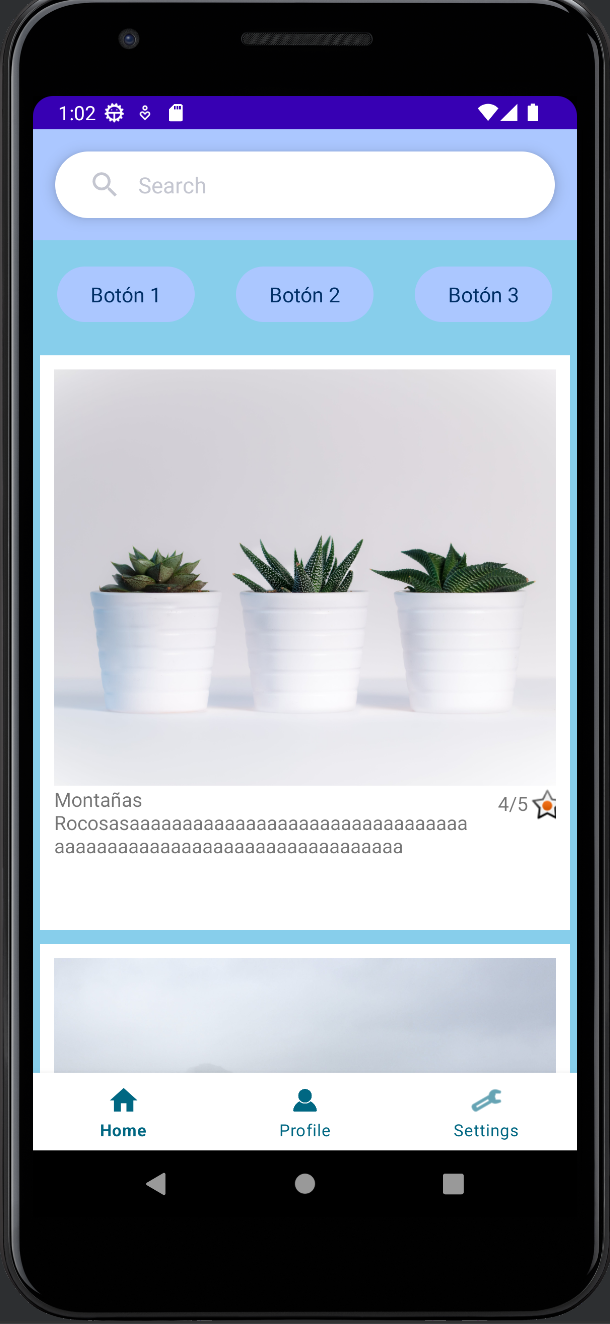
\includegraphics[width=.7\linewidth]{figures/home_dummy.png}
	\caption{Home screen, populated with demo content}
	\label{fig_home_screen}
\end{figure}

\begin{figure}
	\centering
	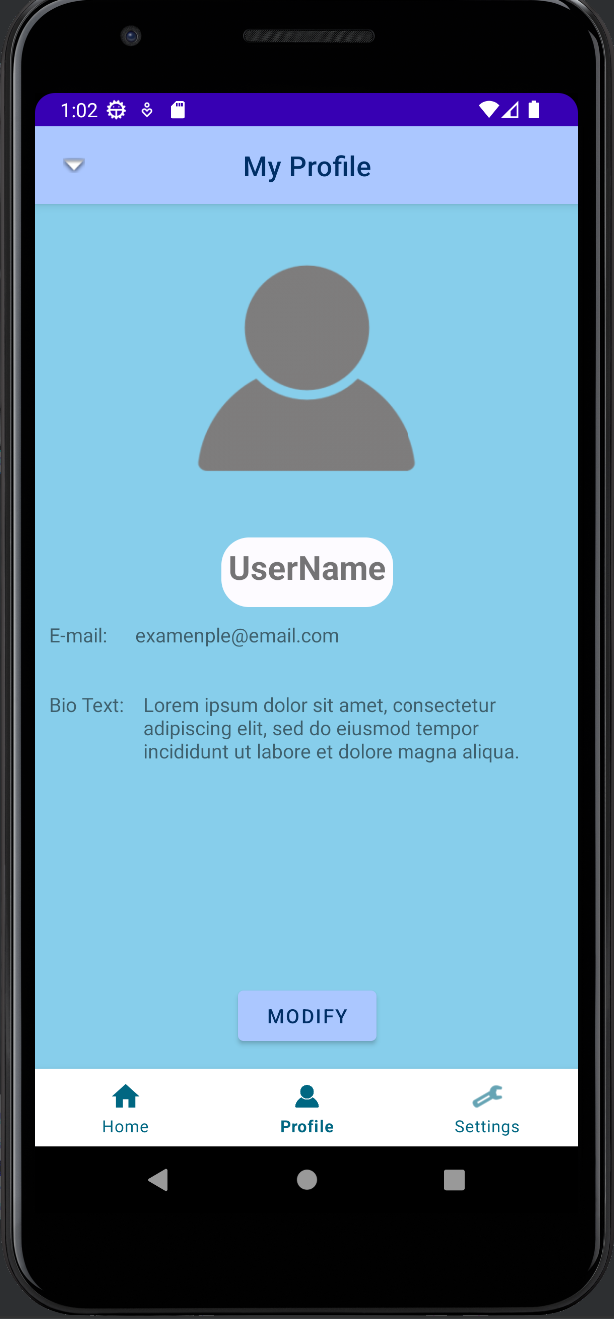
\includegraphics[width=.7\linewidth]{figures/profile_dummy.png}
	\caption{Profile screen with demo content}
	\label{fig:profile_screen}
\end{figure}